\documentclass[11pt,letterpaper]{article}

    %% load packages
    \usepackage[margin=1in]{geometry}       %% document margins
    \usepackage[utf8]{inputenc}
    \usepackage{setspace}                     %% to get \doublespacing command
    \usepackage{authblk}                      %% to get \affil command
    \usepackage{bibentry}                     %% bib formatting
    \usepackage{parskip}                      %% space between paragraphs
    \usepackage{fontspec}                     %% for \setmainfont command, will need xelatex to compile Arial
    \usepackage[comma,super,sort&compress]{natbib}  %% https://latex.org/forum/viewtopic.php?t=8399
    \usepackage{graphicx}                     %% for figures

    %% general document formatting commands
    \pagestyle{plain}                         %% page numbers in middle
    %\linespread{1.67}                        %% baseline linespread = 1.2 (1.2*1.67~2)
    \doublespacing
    \setmainfont{Arial}                       %% https://latex.org/forum/viewtopic.php?t=25998
    \setcitestyle{citesep={,}}
    \graphicspath{{figs/}}                    %% set path to figures relative to this document

    \title{Potential Novel Immunotarget Revealed in Mega Analysis of Colorectal Transcriptomes}

    \author[1]{Christopher H. Dampier, MD}
    \author[2]{David F. Grabski, MD, PhD}
    \author[1]{Matthew Devall, PhD}
    \author[3]{Virginia Diez-Obrero, BS}
    \author[3]{Ferran Moratalla-Navarro, MS}
    \author[4]{David Rekosh, PhD}
    \author[4]{Marie-Louise Hammarskjold, PhD}
    \author[5]{Sara K. Rasmussen, MD, PhD}
    \author[3]{Victor Moreno, MD, PhD}
    \author[1,*]{Graham Casey, PhD}

    \affil[1]{Center for Public Health Genomics, University of Virginia, Charlottesville, Virginia, USA}
    \affil[2]{Department of Surgery, University of Virginia, Charlottesville, Virginia, USA}
    \affil[3]{Catalan Institute of Oncology, Barcelona, Spain}
    \affil[4]{Department of Microbiology, Immunology and Cancer Biology, University of Virginia, Charlottesville, Virginia, USA}
    \affil[5]{Department of Surgery, Seattle Children's, Seattle, Washington, USA}
    \affil[*]{Correspondence: Graham Casey, PhD, Center for Public Health Genomics, MSB Room 3238, Department of Public Health Sciences, University of Virginia, P.O. Box 800717, Charlottesville, VA 22908-0717, gc8r@virginia.edu}

    %% redefine maketitle function to customize title formatting
        %% https://tex.stackexchange.com/questions/85343/left-align-abstract-title-and-authors
        %% https://en.wikibooks.org/wiki/LaTeX/Fonts#Sizing_text
    \makeatletter
    \renewcommand{\maketitle}{
        \begingroup
            \setlength{\parindent}{0pt}
            \begin{flushleft}
                \LARGE\textbf{\@title}
                \newline
                \newline
                \normalsize\@author
            \end{flushleft}
        \endgroup
    }
    \makeatother

\begin{document}

\maketitle

\newpage
\section*{Synopsis}
1 to 3 sentences, no more than 45 words

\newpage
\section*{Abstract}
\textbf{Background}:
Microsatellite unstable, mismatch repair deficient metastatic cancers can be treated with immune checkpoint inhibitors, but new therapeutic approaches are needed to extend the benefits of immune modulators to the majority of patients with microsatellite stable tumors.
Cancer specific over expression of human endogenous retroviral elements could be exploited to enhance immune infiltration of microsatellite stable colorectal cancer and render these tumors more susceptible to immune checkpoint inhibition.
To identify novel targets for immune mediated cancer therapies, we tested for cancer specific over expression of endogenous retroviral transcripts in a large cohort of colorectal transcriptomes.

\textbf{Methods}:
A recently curated RNA sequencing dataset composed of 1,139 human primary colorectal tissue samples divided into three cohorts was re-processed using a novel annotation of repeat element transcripts to quantify levels of repeat element expression in colorectal transcriptomes.
A total of NUMBER healthy, NUMBER tumor-adjacent normal, and NUMBER tumor samples were profiled with short read sequencing.
Transcripts were quantified with Salmon using the GENCODE v36 transcriptome augmented to include unannotated exons from long terminal repeat elements classified as human endogenous retroviruses (HERVs) in the Dfam database.
Associations between transcript expression and tissue phenotype were tested using DESeq2 in the R statistical language.

\textbf{Results}:
Out of 5,025 unannotated HERV genes measured in 834 samples, including NUMBER healthy, NUMBER tumor-adjacent normal, and NUMBER tumor samples, 150 were expressed within one standard deviation of median protein coding gene expression in at least one tissue phenotype.
Over half of the 150 HERV genes with moderate expression were in the H (26) or K (51) classes.
Tumor specific over expression was observed in 11 of the 150 HERV genes tested.

\textbf{Conclusions}: The conclusions go here.

\newpage
\section*{Introduction}
Colorectal cancer (CRC) is a common malignancy in the United States.
Early detection and effective treatment result in a 5-year relative survival of 90\% for patients diagnosed with local disease.
However, over a fifth of new cases are diagnosed with metastatic disease, which has a 5-year relative survival of only 14\% \citep{SEER2020}.
To improve overall survival of patients with distant disease, new therapeutic approaches are needed.

Immunotherapy in CRC is a promising new treatment option for patients with distant disease.
Immune checkpoint inhibition was shown to achieve durable responses with programmed cell death protein 1 (PD-1) antibody monotherapy and combination therapy with antibodies for PD-1 and cytotoxic T-lymphocyte-associated
protein 4 (CTLA-4) \citep{Le2015, Overman2018}.
However, response to immune checkpoint inhibition was limited to the subset of tumors with mismatch repair defficiency and high microsatellite instability, which constitute approximately 4\% of all metastatic CRC cases \citep{Ganesh2019}.
Strategies to improve tumor immunogenicity and increase cytotoxic T cell infiltration are required to help extend the benefit of immune therapies to the other 96\% of metastatic CRC.
Epitopes derived from endogenous retroviral peptides expressed in cancers may offer a solution.

Human endogenous retroviruses (HERVs) are proviral elements integrated into the human genome under conditions that render them incompetent of replication or infection.
Residual HERV elements in contemporary human genomes are the consequence of retroviral infections of germ cells millions of years ago.
Since then, and like the rest of the human genome, HERV elements have accumulated point mutations and segmental deletions.
These alterations in HERV sequences disrupt assembly of functional viral machinery.
Nevertheless, some HERV sequences can still be transcribed and translated, and a subset are processed as endogenous antigens and presented on major histocompatibility complex (MHC) class I molecules \citep{Boller1997, Rooney2015}.
In healthy tissues, DNA methylation and histone modification can silence transcription of HERV genes, but epigenetic modifications in the context of oncogenesis can de-repress HERV transcription and lead to translation of neoantigens \citep{Menendez2004, Wiesner2015}.

The cancer specificity of putative HERV peptides makes them promising biomarkers for and targets of immune therapies.
A major challenge to the development of HERV based therapies is the absence of consensus on how to find HERV gene products.
Proviruses are generally absent from human gene, transcript, and protein annotations, and their structural features make them hard to identify in agnostic surveys based on DNA or RNA sequencing \citep{ERVmap2018, Treangen2011}.
Proviral genomes are flanked by repetitive elements that often cannot be mapped with short read sequencing.
Furthermore, HERVs are transposable elements that have generated many similar proviral integrations throughout the human genome.
The multitude of similar sequences across the genome impairs accurate high throughout read alignment.
As a result, the genomic locations and transcriptional abundances of most HERVs are not known with confidence.

Recently, new approaches have been developed to overcome traditional limitations in HERV annotation, quantification, and protein identification \citep{Attig2017, Attig2019, ERVmap2018, Telescope2019}.
Here, we extend advances in the characterization of HERV transcriptomes to discover novel CRC specific expression patterns.
We test for differential expression of HERV transcripts in a large cohort of healthy, tumor-adjacent normal, and tumor RNA sequencing data and identify HERV transcripts over expressed in tumor samples.
We then predict the neoantigens most likely to succeed as biomarkers and immunogenic peptides in the treatment of CRC.

\section*{Methods}
\subsection*{Sample Selection}
Bulk RNA sequencing (RNA-seq) from a recently curated set of 1,139 flash frozen colorectal tissue samples was re-processed and analyzed for the presence of unannotated HERV genes \citep{Dampier2020}.
For discovery of associations between tissue phenotypes and HERV expression, paired end sequencing from 834 colon biopsies was used.
Of those biopsies, 462 were healthy tissue, 61 were tumor adjacent normal tissue, and 311 were tumors.
These samples are referred to as the discovery cohort.

For validation of discovered associations, two independent cohorts were used.
The first (validation \#1) included paired end sequencing from 30 pairs of tumor and matched adjacent normal biopsies (i.e. 15 samples of both tissue phenotypes paired by subject).
The second (validation \#2) included single end sequencing from 275 colon biopsies of which NUMBER were healthy, NUMBER were tumor adjacent, and NUMBER were tumor.
An important characteristic of the discovery cohort and the validation \#2 cohort was the independence of all tumor and tumor adjacent samples.
To permit valid inference from regular linear models, only one tissue phenotype was used per subject.

Samples were gathered from publicly available RNA-seq datasets hosted on the Genomic Data Commons and Sequence Read Archive as well as from a recently generated dataset of healthy mucosal biopsies obtained during screening colonoscopies at the Catalan Institute of Oncology in Barcelona, Spain \citep{Dampier2020, DiezObrero2020}.
A complete description of sample selection and cohort construction for the curated dataset is available in Dampier et al. \citep{Dampier2020}.
RNA-seq reads for all samples were stored and analyzed in FASTQ format.
For samples downloaded in BAM format, Biobambam2 v2.0.87 \citep{Tischler2014} was used to convert reads to FASTQ format.

\subsection*{Human Endogenous Retrovirus Gene Annotation}
HERVs were identified using the genomic coordinates (GRCh38) and feature names of exons and spliced transcripts of HERV elements from a recently published human cancer transcriptome annotated with the GENCODE v24 basic gene model \citep{Frankish2018} and a model of genome-wide repeat elements \citep{Attig2019}.
The cancer transcriptome was assembled from RNA-seq reads of 24 subjects from each of 32 cancer types obtained from The Cancer Genome Atlas (TCGA), as previously described \citep{Attig2019}.
Names and coordinates of repeat elements were generated using RepeatMasker \citep{Smit2015} configured with nhmmer \citep{Wheeler2013} in sensitive mode using the Dfam 2.0 library (v150923) \citep{Hubley2015}, as previously described \citep{Attig2017}.
The method relies on profile hidden Markov models representing known human repeat families to classify repeat elements throughout the genome.

Previously unannotated HERV genes were selected for the current study in multiple steps.
A complete gene transfer format (GTF) \citep{GTF} annotation of the repeat element inclusive cancer transcriptome was downloaded from Attig et al. \citep{Attig2019}.
The annotation was parsed with a custom Python script to produce a new annotation in BED12 \citep{BED12} format.
Transcripts were selected based on three criteria: i) overlap of at least one exon with a long terminal repeat element, ii) classification of at least one exon as HERV derived, and iii) abscence of any exon overlapping an annotated GENCODE gene.
All transcripts labeled with the same repeat element identifier (i.e. repeat element class along with genomic coordinates) were considered isoforms of the same HERV gene.
Genomic coordinates were extracted for all constituent exons of selected transcripts to permit inference of splice sites and exclusion of intronic sequences.
For display purposes, repeat element identifier genomic coordinates were converted to cytobands.

\subsection*{Transcript Quantification}
Transcript quantification was performed with Salmon v1.2.1 \citep{Patro2017} in mapping-based mode with the \verb|--gcBias| and \verb|--validateMappings| flags set.
Inputs to the Salmon \verb|quant| command were RNA-seq reads in FASTQ format and the Salmon index.
To create the Salmon index, a custom reference transcriptome was built from a list of GENCODE v34  transcript sequences \citep{Frankish2018} and the list of unannotated HERV transcript sequences.
GENCODE sequences were downloaded from the GENCODE FTP site \citep{GENCODE-transcripts}.
HERV sequences were extracted from the GRCh38 reference genome \citep{ENCODE-GRCh38} using the BEDTools \citep{Quinlan2010} \verb|getfasta| command with the \verb|-split| option and the custom BED12 annotation of selected HERV transcripts.
Following the recommendation of Salmon's authors \citep{SalmonDecoys}, contig sequences from the GRCh38 reference genome were subsequently added to the target transcript sequences as decoy sequences to generate a decoy-aware transcriptome for indexing.

\subsection*{Gene Expression Analysis}
Associations between HERV gene expression and tissue phenotype were tested using the \emph{Bioconductor} suite of genomics analysis packages \citep{bioc} in the R statistical programming language \citep{R}.
Specifically, \emph{tximport} \citep{Soneson2015} was used to extract transcript length and abundance estimates from Salmon and summarize them to the gene level for input into \emph{DESeq2} \citep{Love2014}.
Count matrices of HERV and GENCODE genes were prefiltered to select genes with a count of at least one read in at least half of the samples in each cohort.
Factors to normalize counts for sequencing depth and transcript length were calculated with \emph{DESeq2}.
Latent factors of non-biological variation were estimated with \emph{sva} \citep{sva}.
Genes of interest for association testing were selected in several steps.

First, counts of all genes were transformed with the variance stabilizing transformation of \emph{DESeq2} and adjusted for batch effects with \emph{limma} \citep{Ritchie2015}.
Second, adjusted counts of all annotated genes were filtered to retain only protein coding genes.
Third, median and standard deviation of protein coding gene expression were calculated separately for each tissue phenotype in each cohort.
Finally, adjusted counts of HERV genes were filtered to retain only HERVs expressed within a single standard deviation of median protein coding gene expression in at least one tissue phenotype.

Counts of all protein coding genes and HERVs with sufficient expression were modeled with phenotype and latent factors as explanatory variables using \emph{DESeq2}.
Significant associations between gene count and tissue phenotype were identified by testing whether the absolute value of the effect of phenotype was at least two fold change for a given gene.
Multiple hypothesis testing correction was performed using a false discovery rate of 5\%.

\section*{Results}
\subsection*{Over-Expression of Novel HERV Genes in Tumors}
To define an inclusive set of non-canonical HERV elements against which to compare CRC transcripts, we started with a recently published model of the human cancer transcriptome assembled \emph{de novo} from TCGA samples and annotated with \emph{RepeatMasker} using the Dfam database \citep{Attig2019}.
The complete annotation included over 1 million transcripts, 416,862 of which overlapped long terminal repeat sequences (i.e. the repeat sequences that flank HERV genes).
To discover novel, cancer-specific HERV expression, we identified a subset of transcripts composed of exons without GENCODE annotations, at least one of which was classifed as a HERV element.
There were 16,336 transcripts composed of 35,666 exons from 5,025 genes that met our criteria (Figure \ref{fig:ele_sum}A).
To estimate gene abundance, RNA-seq reads from a discovery cohort of 834 colorectal samples were quasi-mapped to a transcriptome composed of GENCODE reference transcripts combined with the 16,336 unannotated HERV transcripts using Salmon.
A total of 150 unannotated HERV genes were expressed at levels within a standard deviation of canonical protein coding genes.
Approximately half were from classes K and H, two of the better characterized classes of HERV (Figure \ref{fig:ele_sum}B).

To identify HERV genes that could encode tumor specific neoantigens, we compared expression levels in tumor samples to levels in healthy samples and histologically normal tumor adjacent samples.




We test for differential expression of HERV transcripts in a large cohort of healthy, tumor-adjacent normal, and tumor RNA sequencing data and identify HERV transcripts over expressed in tumor samples.
We then predict the neoantigens most likely to succeed as biomarkers and immunogenic peptides in the treatment of CRC.


Tumor specific overexpression ... antigenic potential
cohort A
then cohorts B and C
then cohort A without Attig TCGA 48 + 18 (24 COAD tumor, 24 READ tumor, 12 COAD NAT, 6 READ NAT) and GTEx 12
then MSI vs MSS
then tumors with most HERV overexpression
then immunogenic peptide prediction

\subsection*{HERV Genes in Healthy Tissue}

Healthy overexpression ... functional role
cohort A
then cohorts B and C
then Grabski method

\section*{Discussion}

HERVs could be used as immune targets or biomarkers
HERVs may play a role in maintaining healthy epithelium
Limitations
Conclusion

\section*{Acknowledgements}

People we want to thank. Grant support.

\bibliography{main}
\bibliographystyle{vancouver}

\section*{Figure Legends}

Legs

\section*{Tables}

Tabs

\section*{Figures}

\begin{figure}[ht]
  \makebox[\textwidth][c]
  {
    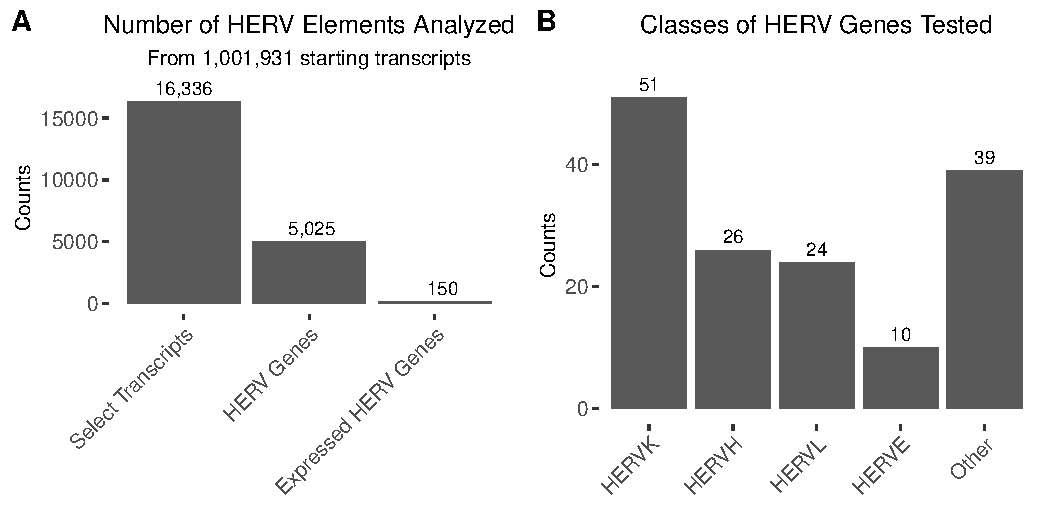
\includegraphics[width=0.9\textwidth]{herv-element-sum_A}
  }
  \caption{Summary of unannotated human endogenous retroviral sequences}
  \label{fig:ele_sum}
\end{figure}


\end{document}

problems with AMA style file...
https://tex.stackexchange.com/questions/55020/updated-ama-bst-file
